
\documentclass[conference]{IEEEtran}
\pagestyle{plain}

\usepackage{amssymb}
\usepackage{xspace}
\usepackage{listings}
\usepackage{siunitx}
\usepackage{balance}
\usepackage{graphicx}
\usepackage{tabularx}
\usepackage{booktabs}

\newcommand{\todo}[1]{\color{red}{\textbf{\em [TODO: #1]}}\xspace}
\newcommand{\TODO}[1]{\todo{#1}}


\ifCLASSOPTIONcompsoc
  \usepackage[nocompress]{cite}
\else
  \usepackage{cite}
\fi


\begin{document}


\newcommand{\FigFragmentSingle}{
\begin{figure}
    \centering
    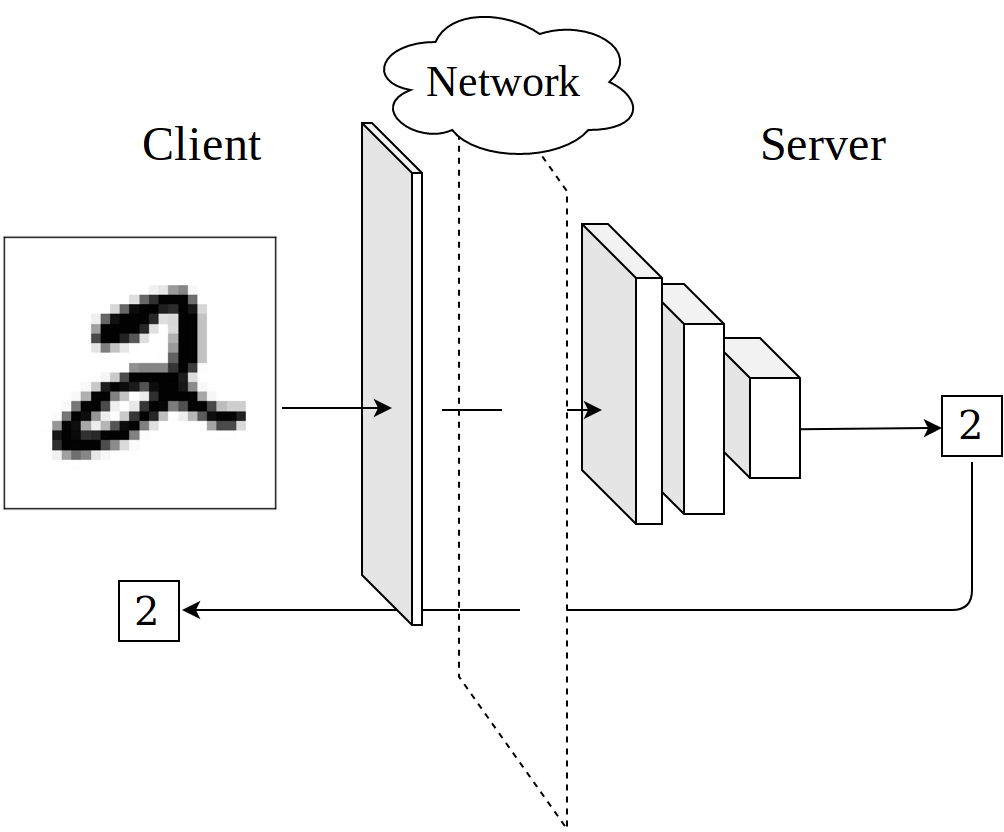
\includegraphics[width=0.4\textwidth]{images/diff_shard_nn-proposed.png}
    \caption{\textbf{Fragmented Machine}\,---\,%
        We propose fragmenting models into two pieces one of which will 
        be distributed to clients. In this way we can rely on the compression
        to latent manifolds to create privacy preserving classification services
        where the service doesn't learn the exact input.}  
    \label{fig:frag-single}
\end{figure}
}


\newcommand{\FigFragmentMany}{
\begin{figure}[t]
    \centering
    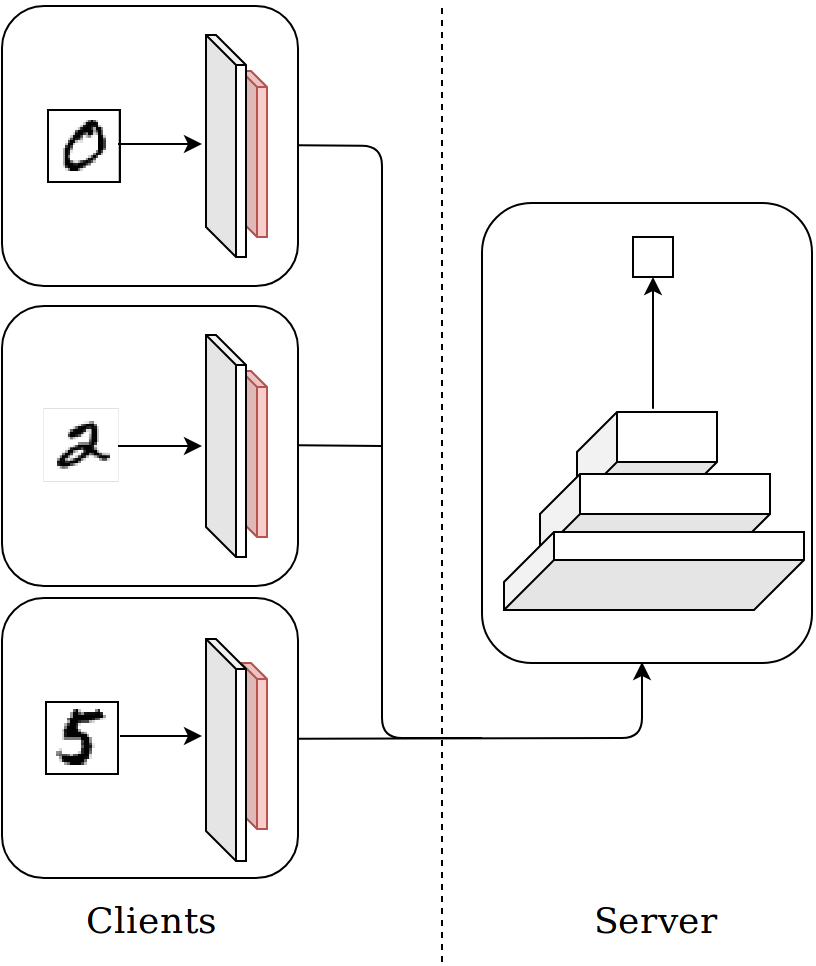
\includegraphics[width=0.4\textwidth]{images/diff_frag_many.png}
    \caption{\textbf{Multi-Party Machine}\,---\,%
        For a service that accommodates many users a fragmented model can distribute
        semi-unique portions of the model to each user. Each client then employs 
        techniques to increase the cost of inverting the model such that a service
        never truly operated on un-encoded data, and translating the data back to it's
        original domain is extremely (approximating prohibitively) expensive.}  
    \label{fig:frag-many}
\end{figure}
}


\title{Just The Facts Please:\\\large Relaxed Differentially Private Classification Techniques for Neural Networks}


\author{\IEEEauthorblockN{Jack Wampler}
\IEEEauthorblockA{School of Electrical, Computer, and Energy Engineering\\
University of Colorado Boulder\\
Email: jack.wampler@colorado.edu}
}
% \and
% \IEEEauthorblockN{Homer Simpson}
% \IEEEauthorblockA{Twentieth Century Fox\\
% Springfield, USA\\
% Email: homer@thesimpsons.com}
% \and
% \IEEEauthorblockN{James Kirk\\ and Montgomery Scott}
% \IEEEauthorblockA{Starfleet Academy\\
% San Francisco, California 96678-2391\\
% Telephone: (800) 555--1212\\
% Fax: (888) 555--1212}}

% make the title area
\maketitle

%\begin{abstract}

% As a general rule, do not put math, special symbols or citations
% in the abstract

The abstract goes here.
\end{abstract}

\section{Introduction}

Many internet services leverage neural networks make classifications on data that consumers
might consider private. However, any data that a user submits may be used in future networks, sold to 
third parties, or redistributed arbitrarily if the service becomes compromised.

With this work we aim to demonstrate that privacy preserving classification can be made by services
which use neural networks by migrating a portion of the learning process to the client. 
Fragmenting the neural network models in this way creates a paradigm where a client is sending 
a low dimensional manifold representation of their data to the service such that the service 
will be unlikely to accurately reconstruct the exact input. 

In concert with this we intend to test other methods for increasing the cost of model
inversion to make it more difficult for an untrustworthy service to reconstruct a
sensitive sample from a user. We consider using probabilistic methods similar to Google's 
RAPPOR project on classification input data while balancing against and classification
errors that this induces. 

While these methodologies are by no means cryptographically secure means of querying a 
neural network service without revealing the input data, we rely in the intuition that a 
a manifold representation of the input optimized for a specific task will prevent direct 
leakage to third parties for unrelated tasks. Similarly if the service becomes compromised, 
either internally or externally, there is no first hand personally identifiable information (PII) 
directly available. 

\subsection{Threat Model}
The thread model that this work adopts relies on a user and a service provider model. The 
service provider gives access a prediction model reliant on a multi-layer neural network 
that was trained on a data-set known to the provider. 
This service can be queried as an oracle by a number of users with (potentially sensitive)
data that they provide. Imagine a network of independent hospitals that would like to use a
prediction service to analyze patient health data - in this scenario there are restrictions
on the ability to share the relevant data based on its sensitivity. 

\section{Architecture}

\FigFragmentSingle

The network modifications that we propose are constructed as follows.

\textbf{Model Fragmentation --}
We propose splitting a trained neural network into two pieces, or designing a neural 
network (recurrent or otherwise) to have two pieces, one of which can be transferred
to the client. When a users wishes to make use of the classification of the service they
first process their input through the piece of the model locally to translate the input
to a low dimensional manifold representation that is (theoretically) specially trained
for the one specific classification task. This pre-processsing the on the client side 
creates a barrier to translating an input to an unrelated task by essentially compressing
the input to relevant features. This can also be thought of as an encoder on the client
side, giving every client an ability to balance computational expense against privacy 
concerns.


\textbf{Model Inversion Resistance --}
To further protect the privacy of user data we attempt to increase the difficulty of
model inversion attacks. That is, a service provider who receives a low order 
representation input from a user should not be able to restore that input to full
fidelity outside of the context of the classification task that they are performing. 
We attempt to increase the difficulty of this task while maintaining the fidelity of
of the classification overall. To this end we will investigate the addition of stochastic
noise, and/or probabilistically dropping features from the input vector -- operations 
which are not easily reversed with high accuracy.

\medskip
Our intention is to design these constructions such that they can be applied generically
to arbitrary neural networks models. In this way we construct models for arbitrary
classification tasks, or adjust existing modes, such that a user is able to make 
classifications under relaxed differentially private gurantees.


\section{Evaluation Metrics}

We aim to demonstrate a task agnostic property of this technique by evaluating its effect 
on various models accomplishing disparate tasks. This can include image recognition tasks
such as MNIST or Imagenet, language comprehension tasks such as machine translation or 
text summarization, or tasks in alternative domains such as medical diagnostics or advertising.

We intend to measure the ability of the service provider to invert the fragment of the model 
that the client possesses using maximum a posteriori (MAP) estimators~\cite{fredrikson2015model}, 
variational autoencoders~\cite{doersch2016tutorial}, or other techniques.

To evaluate the efficacy and efficiency of the techniques outlined above we intend to compare
performance of this method on both the client and service provider. Performance elements include
classification delay, operations per second on both user and service provider, network 
load (i.e. size and frequency of communications), and theoretical throughput for a service 
that requires near real time data. 
\section{Related Work}

The work attempts to address a different from Papernot \textit{et. al.} as they evaluate the ability to
train a neural network on differentially private data~\cite{papernot2016semi}. We instead rely on a network
that has already been trained and attempt to secure the inputs to that network from an untrusted service
provider. We also not that this method is fundamentally different from Bonawitz \textit{et. al.} as their 
technique seeks to accomplish secure, differentially private aggregation of data only using multi-party
computation~\cite{bonawitz2017practical}.

In this work we adopt a similar motivation to private classification techniques like Gilad \textit{et. al.} and 
Chou \textit{et. al.} however we propose removing the requirement for cryptographic assurance of privacy 
making performance and limited trust defining characteristic
differences~\cite{gilad2016cryptonets,chou2018faster,chabanne2017privacy}. The relaxed constraints
of model fragmentation based techniques give a major enhancement over homomorphic models as machines 
can be arbitrarily complex with no depth limitation. This explodes the number of tasks that can be 
accomplished privately without significantly increasing the overhead of the machine. 


Other related work~\cite{yuan2014privacy,barni2006privacy,orlandi2007oblivious,chen2009privacy}

\FigFragmentMany


%% use section* for acknowledgment
% \ifCLASSOPTIONcompsoc
%   % The Computer Society usually uses the plural form
%   \section*{Acknowledgments}
% \else
%   % regular IEEE prefers the singular form
%   \section*{Acknowledgment}
% \fi


\bibliographystyle{IEEEtranS}
\bibliography{biblio}

\end{document}